\section{Introduzione}

\subsection{Motivazioni}

\subsubsection{Storia}
Negli ultimi decenni, l'evoluzione della robotica ha conosciuto un'accelerazione senza precedenti, trasformando ciò che un tempo era materia esclusiva della fantascienza in una concreta realtà industriale e sociale. Tra le molteplici declinazioni della robotica, i robot umanoidi occupano un ruolo di particolare rilievo per il loro potenziale simbolico, funzionale e relazionale. Progettati per imitare forma, movimenti e talvolta comportamenti dell'essere umano, incarnano l'ambizione di rendere il lavoro di quest'ultimo meno faticoso, pericoloso e alienante. 

Sin dall'antica Grecia\footnote{Filone di Bisanzio nel III secolo a.C. descrive meccanismi automatici e figure animate idraulicamente.} la fantasia dell'uomo è solleticata dall'idea di creare un automa a sua immagine e somiglianza, una "creatura" che superasse i limiti umani pur mantenendone le sembianze. Questo desiderio percorre la storia stimolando l'ingegno di Leonardo da Vinci\footnote{progetta un "cavaliere meccanico" capace di compiere movimenti basilari.} e ispirando Karel Čapek che, nella sua opera "R.U.R.\footnote{sigla di \textit{Rossumovi univerzální roboti}, traducibile dal ceco come "robot universali di Rossum"}" del 1921, utilizza per primo il termine \textit{robot} riferendosi proprio a degli automi antropomorfi\cite{wikipediaRUR}. La svolta che porta all'inizio della disciplina robotica per come la intendiamo oggi è la realizzazione di Elektro\cite{wikipediaElektro}, un robot umanoide costruito da Westinghouse, presentato alla Fiera Mondiale di New York. Ovviamente, quando si parla di robotica umanoide non si può non citare Isaac Asimov che formalizza le Tre Leggi della Robotica\cite{britannicaThreeLaws} nel 1950, influenzando la cultura e l'etica della disciplina. Solo un anno dopo viene impiegato il primo robot industriale\cite{avizzano2005robotica} presso la Commissione Energetica Atomica in Francia; si tratta di un pantografo\footnote{manipolatore teleoperato dotato di giunti} meccanico usato per manipolare a distanza il materiale radioattivo senza il coinvolgimento diretto dell'essere umano. In Giappone, nel 1973, l'Università di Waseda realizza WABOT-1\cite{wabotHistory}, il primo robot umanoide capace di camminare, manipolare oggetti e comunicare in giapponese semplice. Circa tredici anni dopo Honda avvia il suo progetto E0 che vedrà la nascita di ASIMO\cite{wikipediaAsimo} in Figura \ref{fig:ASIMO}, presentato al mondo nel 2000, capace di camminare, correre e interagire con l'ambiente in modo autonomo. I primi anni del XXI secolo segnano l'epoca della robotica sociale; l'interesse principale della ricerca si sposta dalla locomozione e dall'esecuzione di compiti manuali alla capacità di rapportarsi al contesto umano in maniera fluida e coerente. Gli alfieri di questo cambiamento sono Pepper di SoftBank\cite{pepperSoftbank2025} e Sophia di Hanson Robotics\cite{sophiaHanson2025} che per primi vengono progettati per relazionarsi con l'essere umano con naturalezza. Gli ultimi cinque anni hanno visto la crescita dell'integrazione tra robot umanoidi ed AI conversazionale e l'affermarsi dell'apprendimento continuo in tempo reale, grazie all'uso di reti neurali profonde.

\begin{figure}[h]
    \centering
    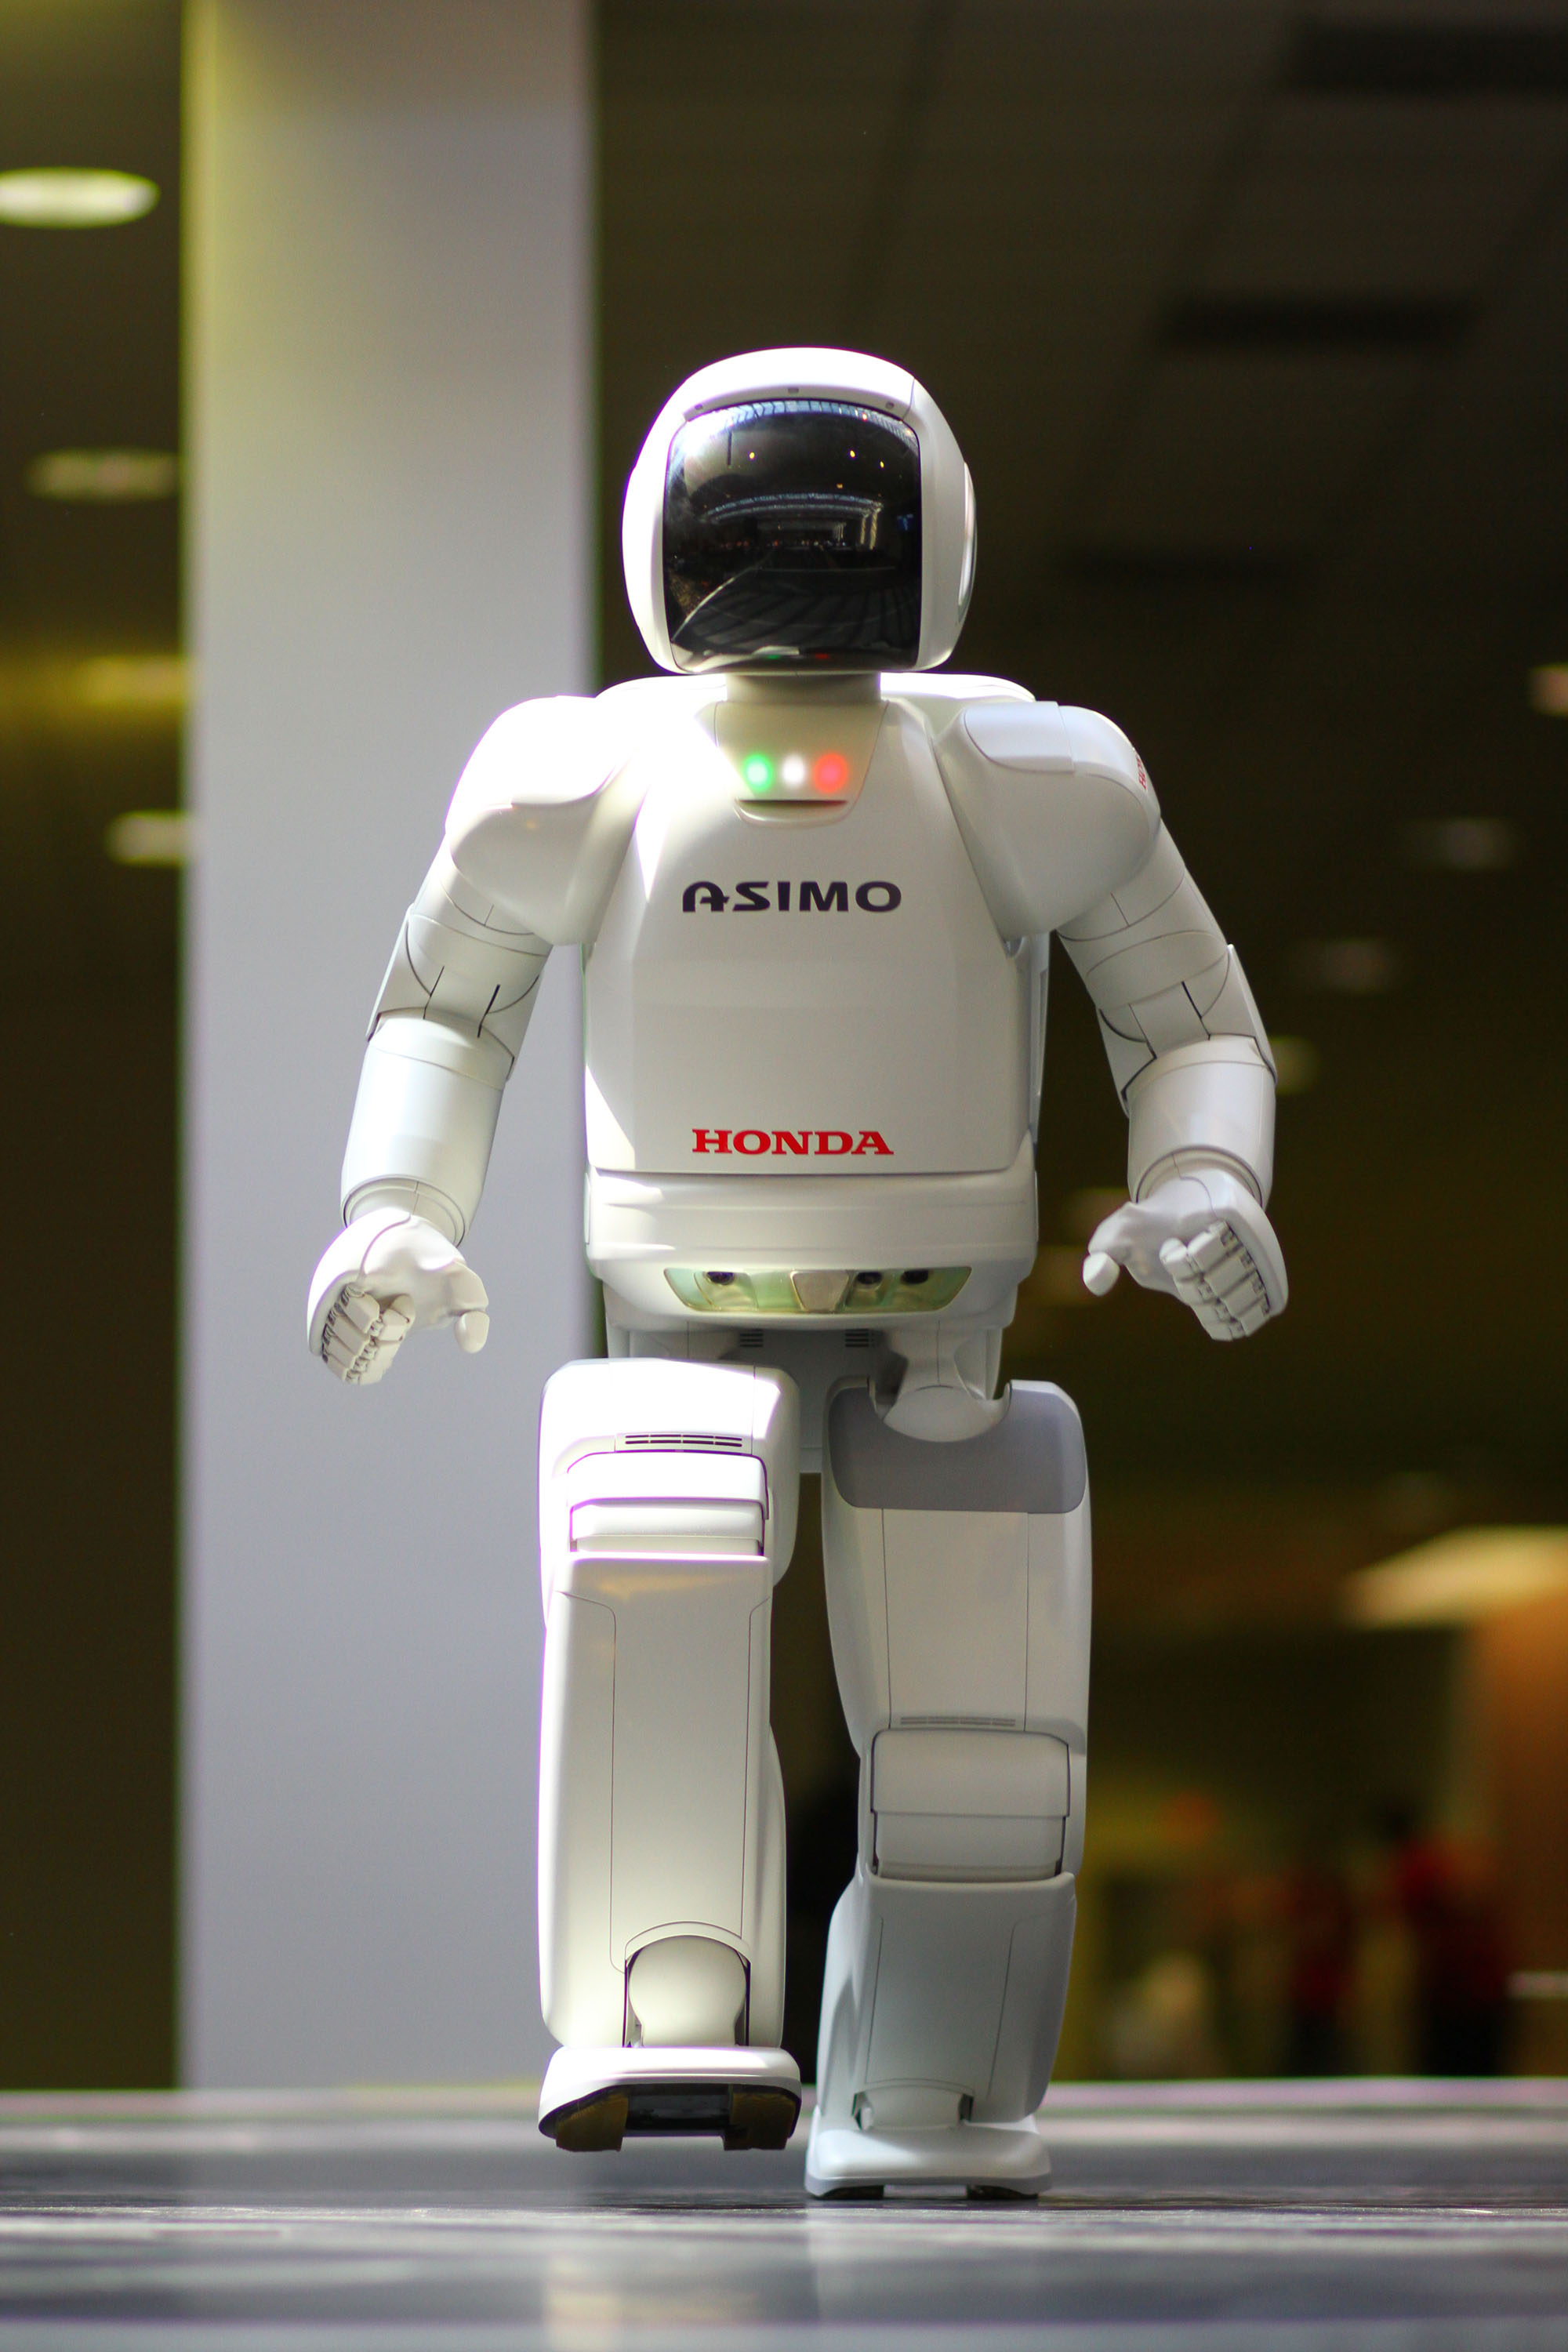
\includegraphics[width=0.35\linewidth]{immagini/ASIMO.jpg}
    \caption{Il robot Asimo di Honda. Fonte: \cite{wikipediaAsimo}}
    \label{fig:ASIMO}
\end{figure}

\subsubsection{Interesse attuale}
L'andamento delle vendite dei robot umanoidi negli ultimi anni riflette l'evoluzione di questa tecnologia, che da prototipo sperimentale è divenuta progressivamente un prodotto commerciale, seppur ancora di nicchia. Dopo la pandemia del 2020, l'attenzione alla robotica autonoma è tornata a crescere, trascinata dallo slancio dettato dalla nuova frontiera LLM e, in generale, dal rinnovato interesse per l'AI. 

La Commissione Nazionale per lo Sviluppo e le Riforme della Cina ha appena annunciato investimenti in robotica industriale per 138 miliardi in 20 anni\cite{ifr2023} e si prevede che gli umanoidi rappresenteranno una porzione rilevante di quota. L'Occidente insegue grazie ai privati del settore; Boston Dynamics, Agility Robotics e Tesla dominano il mercato americano. Atlas, il robot umanoide del primo è in fase di test negli stabilimenti di Hyundai Motor Group, Digit, quello di Agility, è impiegato da Amazon per compiti logistici. Tesla ha, d'altro canto, presentato lo scorso ottobre la terza versione di Optimus che sta testando nei propri stabilimenti, prevedendo l'inizio della produzione di massa nel 2026 secondo uno studio \cite{actuia2025} di Bank of America. Viene stimato, inoltre, che nei prossimi anni i costi di produzione di questi automi scenderanno rapidamente da \$ 35000 a \$ 17000 raggiungendo lo stato dell'arte cinese in questo ambito\footnote{l'azienda cinese Unitree commercializza il modello G1 a partire da \$ 16000}. Ciò renderà i robot umanoidi molto più accessibili e aperti allo sviluppo indipendente. L'istituto bancario statunitense prevede, inoltre, che il $65\%$ di questi robot polivalenti sarà utilizzato in ambienti domestici, il $32\%$ nel settore dei servizi e il $3\%$ nell'industria. Questa ripartizione mostra uno spostamento degli usi verso funzioni di assistenza alla persona e di automazione delle attività quotidiane, piuttosto che verso l'industria manifatturiera, tradizionalmente dominata da robot non umanoidi utilizzati per compiti specifici\cite{bofa2025}. Morgan Stanley, in una ricerca \cite{morganstanley2025humanoids} del maggio 2025, sostiene che nei prossimi venticinque anni ci sarà un mercato di 4,7 trilioni di dollari per gli umanoidi, la maggior parte dei quali in ambito industriale, ma anche come accompagnatori o assistenti domestici. Nel report viene anche ipotizzato che entro il 2050 saranno commercializzate un miliardo di unità. 

Secondo fonti autorevoli come Goldman Sachs\cite{goldman2024humanoids} e McKinsey $\&$ Company\cite{mckinsey2021futurework} l'evoluzione nel campo della robotica umanoide andrà nella direzione di una maggiore autonomia cognitiva e fisica, una maggiore accessibilità economica che porterà alla diffusione domestica e, conseguentemente, all'integrazione nella società civile degli automi. Stimano, inoltre, che l'adozione di sistemi robotici avanzati, come gli umanoidi, accelererà in settori con carenza di manodopera o compiti ripetitivi. 


\subsubsection{Rischi ed opportunità}
Che sia in atto una rivoluzione dal punto di vista industriale, sociale ed economico è innegabile (e inevitabile) ma questo non può indurci ad affrontarla con passività o con cieco ottimismo. Anzi, è necessaria, addirittura urgente, una discussione critica, attenta e partecipata in merito alla robotica ed al suo rapporto con l'uomo. Negli ultimi anni sono emersi numerosi studi di settore che evidenziano le criticità e le questioni da dirimere. Per la presente trattazione si è scelto come riferimento un articolo della Mississippi State University \cite{neupane2024security} che affronta la questione dividendola in tre sezioni:
\begin{itemize}
    \item Possibili superfici d'attacco dei sistemi robotici: occorre considerare i rischi di manipolazioni esterne, volontarie e non, del hardware e del software. Ne sono esempi rispettivamente l'alterazione della percezione dei sensori tramite \textit{jamming}\footnote{accecamento dei sensori visivi tramite fasci di luce intensa} e gli attacchi di \textit{spoofing}\footnote{attacco informatico che prevede la falsificazione dell'identità allo scopo di manipolare i dati in una comunicazione tra soggetti autenticati}. Nei sistemi robotici che implementano dei modelli AI va presa in considerazione anche la possibilità di manomissioni in fase di training e di inferenza.
    \item Considerazioni etico-legali: il sempre crescente impatto delle tecnologie robotiche sulla società ha imposto la necessità di definire i confini del giusto e del lecito, quindi di un inquadramento etico e legale. In questa direzione nasce la disciplina della roboetica e vengono prodotte le prime leggi che regolano principalmente il trattamento dei dati personali come il California Consumer Privacy Act (CCPA) negli USA ed il General Data Protection Act (GDPR) in Unione Europea. Non sono ancora previste delle vere e proprie leggi che regolamentano in rapporto uomo-AI oltre quelle appena descritte. Invece, la produzione saggistica sull'impatto etico di questa rivoluzione è molto florida e raccoglie pareri autorevoli e, tra loro, discordanti. Ad esempio si contrappone la visione umano-centrica del progresso robotico di Benanti \cite{BenantiMaffettone2024} a quella molto più critica di Zuboff \cite{Zuboff2019}.
    \item Studi sulla sicurezza dell'interazione uomo-macchina\footnote{provenienti dal filone ci ricerca Human-Robot Interaction (HRI)}: il progredire delle interazioni umano-robot, sia da un punto di vista numerico che della varietà, è accompagnata dall'interesse di analizzarle dal punto di vista fisico, cognitivo e sociale. Lo scopo è comprendere le vulnerabilità e le lacune dei due interlocutori con l'obiettivo di riuscire ad avere un rapporto sicuro, fluido e collaborativo. 
\end{itemize}

In conclusione, secondo il rapporto \cite{neupane2024security} gli sviluppi che determineranno il futuro della robotica intelligente interessano la riduzione delle superfici di attacco, la sicurezza degli ecosistemi in cui avvengono collaborazioni uomo-robot, l'\textit{explainability}\footnote{ambito di ricerca che mira a rendere i modelli AI più trasparenti e comprensibili agli umani} e la standardizzazione della sicurezza tramite valutazione e validazione dei sistemi.

\subsection{Ambito della trattazione}
\subsubsection{Locomozione bipede}
Una delle sfide più interessanti della robotica moderna è fornire agli automi mobili la capacità di esplorare e interagire con l'ambiente circostante. La mobilità interessa diversi domini come aria, terra e acqua e viene resa possibile tramite ruote, cingoli, eliche, gambe e molto altro. Nella trattazione ci si interesserà della locomozione su gambe che emula la deambulazione umana e risulta essere tra le più complesse. Ad oggi la maggior parte dei robot bipedi riesce a muoversi agilmente solo in scenari noti molto controllati; pochi prototipi sono in grado di muoversi in maniera naturale e sicura in ambienti complessi o incerti. Secondo una review \cite{xie2020review} del 2020 le difficoltà maggiori nello svolgimento di questa attività sono le asperità del terreno, i disturbi, le sollecitazioni esterne e le incertezze dei sensori e degli attuatori. Queste criticità al momento tagliano fuori gli umanoidi da tutti i compiti con richieste di velocità o stabilità; pur avendo acquisito una buona fluidità nel camminare in piano, i robot bipedi non sono ancora in grado di correre e saltare in scenari imprevisti. Negli anni il superamento dei terreni impervi è stato l'obiettivo di diversi progetti come la serie HRP di Honda, MABEL dell'Università del Michigan e ATRIAS dell'Università Statale dell'Oregon. I relativi prototipi avevano l'ambizione di conservare robustezza nella camminata nonostante dislivelli, scalini o piccole asperità\footnote{nell'ordine delle decine di centimetri}; la stabilità ottenuta è limitata a velocità ridotte. 


\subsubsection{Evitamento degli ostacoli}
Nell'ambiente in cui opera il robot possono essere presenti oggetti previsti o non che vanno del tutto aggirati; evenienza non presa in considerazione dalle soluzioni proposte sopra. A seconda del caso in esame, il robot può essere consapevole o meno della presenza degli oggetti che si frappongono tra sé ed il punto di arrivo. Se il robot conosce la posizione degli ostacoli, il suo compito è quello di trovare, se esiste, un percorso fattibile fino all'obiettivo; altrimenti è necessario definire un problema di \textit{obstacle detection} da risolvere mentre il robot esplora. Questo compito richiede di raccogliere dati dai sensori esterocettivi, costruire una stima della mappa sulla base di questi e della \textit{belief}\footnote{la posa attesa del robot stimata dall'algoritmo di localizzazione}, confrontare questa con la mappa reale nota e comprendere se la discrepanza tra di esse evidenzia la presenza di ostacoli inattesi. Infine, occorre ripianificare la traiettoria in maniera coerente con l'obiettivo prefissato della navigazione e con la nuova mappa aggiornata. Le strategie per attuare l'\textit{obstacle avoidance} si basano, quindi, sull'ottimizzazione del compromesso tra: obiettivo generale, velocità e cinematica del robot e rischio di collisioni. Nei casi più complessi gli ostacoli sono in movimento oppure è richiesto interagire con essi per superarli come nel caso di scale o oggetti da arrampicare.


\subsubsection{Apprendimento per rinforzo}
Il reinforcement learning rappresenta un approccio particolarmente efficace per affrontare compiti complessi in cui un agente deve imparare a prendere decisioni ottimali attraverso l’esperienza diretta. Uno degli ambiti in cui si dimostra particolarmente utile è quello della robotica, dove viene impiegato, ad esempio, per l’evitamento degli ostacoli, la locomozione autonoma e la manipolazione di oggetti. Tuttavia, i suoi vantaggi si estendono ben oltre, coinvolgendo settori come i videogiochi, dove consente lo sviluppo di agenti in grado di adattarsi a dinamiche di gioco complesse, o la finanza, dove può ottimizzare strategie di investimento attraverso la massimizzazione dei profitti nel lungo termine. Anche nei trasporti, l'apprendimento per rinforzo è alla base di sistemi di guida autonoma capaci di affrontare situazioni imprevedibili nel traffico, mentre nella gestione energetica o nelle reti informatiche può aiutare a distribuire le risorse in modo efficiente. In generale, la forza di questo approccio risiede nella sua capacità di apprendere politiche di comportamento efficaci in ambienti dinamici e incerti, migliorando con l’esperienza e adattandosi in tempo reale a nuove condizioni senza necessità di una programmazione esplicita.


\subsection{Obiettivi}
\subsubsection{Intenzioni}
La presente trattazione si propone di sviluppare un modello di reinforcement learning in grado di interpretare le osservazioni provenienti da sensori esterocettivi e propriocettivi di un robot umanoide e controllarne i giunti al fine di eseguire compiti di locomozione in ambienti con ostacoli. La buona riuscita del compito passa da una valida contestualizzazione teorica e da una scelta consapevole delle tecnologie da impiegare. La progettazione non può, quindi, che iniziare con la ricerca dell'algoritmo più adatto per lo scenario proposto. Dal punto di vista teorico, la natura \textit{data-driven} del reinforcement learning impone un numero di esperienze e una variabilità degli scenari che solo la simulazione via software può garantire. Inoltre, l'addestramento diretto nella realtà porrebbe limiti insormontabili in termini energetici, di tempo e di sicurezza dell'automa. Risulta, quindi, naturale dividere il processo di sviluppo in una fase di training in simulazione e una, successiva, di implementazione reale che prevede la traduzione della politica ottenuta al passo precedente in un vero e proprio algoritmo di controllo robotico.

\subsubsection{Scenari di addestramento}
La caratteristica fondamentale degli algoritmi basati sul reinforcement learning è la generalizzazione, ossia la capacità di esprimere una politica prestante in scenari sconosciuti e diversi tra loro. Non è di interesse sviluppare un modello in grado di svolgere perfettamente il compito solo nelle condizioni su cui è stato addestrato. Risulta, invece, molto più utile che il modello apprenda le informazioni ad alto livello e i pattern sottesi al rapporto tra le osservazioni che raccoglie e la migliore azione da intraprendere. Ciò permette di confrontarsi con la realtà, la sua variabilità e le sue complesse non idealità. Per ottenere questa capacità è indispensabile fornire alla rete neurale degli ambienti di addestramento complessi e variabili; questo è essenziale per evitare che essa impari lo specifico scenario invece di maturare una comprensione generale del compito. Nel caso preso in esame, si è scelto di procedere per gradi e articolare l'addestramento in tre fasi di difficoltà crescente:

% tre scenari

\subsubsection{Possibile implementazione reale?}
% possibile implemetazione reale


\subsection{Stato dell'arte}
Il recente slancio dell'intelligenza artificiale e l'ingresso sul mercato di robot umanoidi a costi ridotti hanno stimolato una florida produzione di studi relativi alla progettazione di algoritmi di navigazione robotica \textit{AI driven}. Questo permette un'ampia visione sulle possibili soluzioni al problema e sugli aspetti metodologici dell'addestramento e dell'implementazione di tali algoritmi su sistemi robotici complessi. 


\subsubsection{Algoritmi deterministici basati su ostacoli noti}
Una delle implementazioni più semplici di un algoritmo di evitamento degli ostacoli è quella trattata nell'articolo del 2007 di Ching-Chang Wong et al. \cite{wong2007design}. L'obiettivo del team dell'università taiwanese era quello di permettere ad un robot umanoide dotato di un set di sensori infrarossi di procedere verso un'area prefissata evitando ostacoli sconosciuti. La soluzione implementata prevede un albero di decisione usato per selezionare, in base alla posizione relativa dell'ostacolo, la migliore azione da compiere: procedere dritto, curvare di 30° oppure spostarsi lateralmente. Il risultato è una tabella che mette in relazione sedici possibili scenari di rilevamento ostacoli\footnote{di fronte, di lato, multipli, etc...} con la migliore azione da compiere nella circostanza.

\begin{figure}[h]
    \centering
    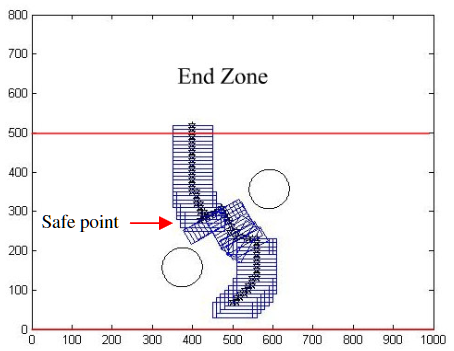
\includegraphics[width=0.35\linewidth]{immagini/simple_OA_IR.png}
    \caption{Percorso del robot tra due ostacoli. Fonte: \cite{wong2007design}}
    \label{fig:simple_ao}
\end{figure}

Nella figura \ref{fig:simple_ao} è visibile come il robot, sin dalle prime fasi, rilevi l'ostacolo a sinistra e cerchi di aggirarlo curvando per poi individuare l'ostacolo a destra e attuare la manovra per passare tra i due. Questa soluzione risulta piuttosto robusta, ma non affronta in nessun modo il tema dell'ottimalità né dal punto di vista della distanza percorsa né da quello del tempo impiegato. Inoltre, la scarsa varietà di possibili azioni non lo rende scalabile a scenari più avanzati.


\subsubsection{Reinforcement learning basato su ostacoli noti}
Le prime implementazioni di reinforcement learning nell'ambito robotico sono nate per compiti come il \textit{pick and place}\footnote{prendere un oggetto e posizionarlo dove richiesto} per i manipolatori, la guida lungo un tracciato per i robot con ruote o cingoli e la camminata fluida per quelli su gambe o zampe. Una volta raggiunto questo obiettivo, l'interesse si è rivolto, nel caso dei robot mobili, alla navigazione di una mappa evitando ostacoli noti. La richiesta era, dunque, quella di imparare a formulare percorsi fattibili nella mappa che raggiungessero l'obiettivo senza colpire gli oggetti presenti nell'ambiente e, dunque, attuare quanto pianificato. Lo studio di M. Hamze, M. Morisawa e E. Yoshida \cite{hamze2024learning} esemplifica bene questo genere di utilizzo del RL. Viene, infatti, coinvolta una rete neurale che fa inferenza sulla posizione del robot e sulla mappa provvista di ostacoli e di posa da raggiungere. L'uscita della rete invia segnali ad un controllore PD che comanda i giunti. Nell'addestramento per rinforzo descritto nell'articolo vengono definite delle ricompense per il raggiungimento dell'obiettivo e per l'evitamento degli ostacoli allo scopo di ottenere una rete capace di ottimizzare il percorso. Viene osservato che l'algoritmo funziona correttamente se gli ostacoli vengono spostati leggermente rispetto a dove erano previsti, mentre il loro riposizionamento casuale inficia pesantemente la robustezza del sistema. Si arriva alla conclusione che per questa fattispecie di compito sia richiesto l'ausilio della sensoristica. L'articolo risulta comunque utile per la comprensione del rapporto tra reinforcement learning e locomozione bipede.


\subsubsection{Reinforcement learning basato su ostacoli ignoti}
La navigazione robusta in scenari non completamente noti rappresenta un passaggio fondamentale nel percorso verso la completa integrazione della robotica nel mondo reale. Gli scenari in cui tutta la mappa è nota e non ci sono elementi di incertezza appartengono ad un numero ristretto di casi d'uso. Risulta sicuramente più interessante capire come permettere al robot che naviga nell'ambiente di individuare gli ostacoli imprevisti e riuscire a reagire correttamente. Per fare ciò è necessario dotare l'automa di una sviluppata capacità di generalizzazione e interpretazione delle osservazioni della scena. Una delle possibili modellazioni di questa situazione è lo \textit{zero-shot learning} (ZSL) che rappresenta lo scenario in cui il modello viene addestrato a riconoscere e categorizzare oggetti o concetti senza averne visto prima alcun esempio. Lo studio di riferimento in merito è stato elaborato da Escontrela, Alejandro, et al. \cite{escontrela2020zero} che propongono l'utilizzo di \textit{Multi-task reinforcement learning} (MTRL), un approccio che mira ad addestrare politiche generalizzabili che possono risolvere un'ampia varietà di compiti. Nell'articolo si spiega come la chiave di una corretta generalizzazione sia la variabilità degli ambienti imposti all'agente. Gli autori hanno ottenuto ciò introducendo entità come scale, buche, ostacoli e terreni dissestati e fornendo ad essi dei parametri aleatori corrispondenti a densità delle asperità, profondità delle buche, altezza degli scalini e ingombri degli ostacoli. Inoltre, per analizzare il contributo di ciascuna componente, viene proposto uno studio di ablazione\footnote{rimozione programmata di componenti del modello per verificare la variazione delle prestazioni} in cui gli autori hanno sostituito il proprio modello MTRL con uno reattivo riscontrando un calo delle performance tra il 21 \% ed il 218 \%. Anche la rimozione del comparto percettivo\footnote{LiDAR in questo caso} ha dimostrato pessimi risultati. Infine, viene diminuita la variabilità ambientale ottenendo un evidente calo dei successi dovuto al \textit{catastrophic forgetting} che si verifica quando un sistema di apprendimento dimentica in modo significativo le informazioni precedentemente apprese a causa dell'acquisizione di nuove conoscenze, come spiegato nel relativo articolo \cite{mccloskey1989catastrophic}. Questo avviene quando le reti vengono addestrate in sequenza, e il nuovo apprendimento interferisce drasticamente con quello vecchio.

% Deep Q-Network vs Proximal Policy Optimization
Uno degli studi più rilevanti nell'ambito della navigazione basata sulla visione è sicuramente quello prodotto per la conferenza \textit{IEEE international conference on robotics and automation} del 2021 \cite{wenzel2021vision}. Vengono citate le limitazioni dello SLAM\footnote{Simultaneous Localization and Mapping, algoritmi di mappatura ed esplorazione simultanea che permettono al robot di navigare scenari ignoti, mapparli e stimare la propria posa} classico e proposti due algoritmi di deep reinforcement learning come possibili soluzioni: \textit{Deep Q-Network} (DQN) e \textit{Proximal Policy Optimization} (PPO). Risulta degna di nota la dissertazione intorno alla definizione dello spazio d'azione del robot e, in particolare, la differenziazione tra spazio continuo e discreto. Secondo l'articolo, utilizzare uno spazio d'azione discreto porta  migliori performance; ciò deriva dal fatto che la rete deve apprendere una relazione tra la velocità lineare e angolare per il dominio continuo mentre, nel dominio discreto, la conoscenza preliminare di questa relazione è già disponibile. Dal punto di vista della percezione, lo studio confronta le prestazioni dell'algoritmo con tre equipaggiamenti:

\begin{itemize}
    \item Immagini in scala di grigi: le osservazioni utilizzabili consistono nelle sole immagini catturate dalla telecamera.
    \item Profondità stimata: a partire dalle immagini viene stimata la profondità grazie ad una rete GAN\footnote{Generative Adversarial Network, rete neurale convoluzionale che sfrutta due sottoreti concorrenti per migliorare l'addestramento, spesso usate nella generazione di immagini e mappe di profondità} addestrata in precedenza.
    \item Profondità reale: vengono fornite all'agente osservazioni effettivamente provenienti da un sensore di profondità
    \item Combinazione di immagini e profondità stimata (\textit{fused}): le immagini e le profondità stimate ricavate da esse vengono combinate e utilizzate insieme come osservazioni da fornire all'agente.
\end{itemize}

Dai risultati sperimentali emerge che avere la profondità reale ottiene le prestazioni migliori in termini di ricompense ottenute, segue la soluzione \textit{fused} che risulta vantaggiosa rispetto ad avere solo immagini o solo profondità stimate.

\subsubsection{Reinforcement learning basato su ostacoli in movimento}
Fino a questo punto della trattazione, gli ostacoli da superare si sono presupposti fissi, ma è molto interessante osservare le soluzioni a problemi più complessi come quelli che prevedono oggetti in movimento nella scena. L'articolo \cite{holgadoalvarez2025dynamicobstacleavoidancebounded} riporta come, per simulare questo scenario, sia necessario implementare due agenti \textit{soft actor-critic}\footnote{algoritmo che impara a comportarsi in modo ottimale cercando il compromesso tra sfruttamento (massimizzazione della ricompensa) ed esplorazione (massimizzazione dell'entropia).}: uno protagonista che controlli il robot ed uno avversario che determini i movimenti dell'ostacolo. Il robot in questo caso è il Go1 di Unitree, un quadrupede provvisto di sensori RGB-D e LiDAR. Per modellare la capacità dell'avversario, gli autori dello studio hanno fatto ricorso alla teoria del \textit{quantal response equilibria} (QRE), ossia una generalizzazione dell'equilibrio di Nash che cerca di bilanciare le probabilità delle azioni che producono ricompense positive e penalizzare prevalentemente gli errori più gravi, facilitando la ricerca di politiche di navigazione efficaci. Il metodo utilizzato viene battezzato dagli ideatori \textit{Hierarchical policies via Quantal Response Adversarial Reinforcement Learning} (Hi-QARL) e, secondo i risultati sperimentali, funziona correttamente quando l'ostacolo in movimento è unico.

Un'altra pubblicazione rilevante in merito è quella della University of Auckland \cite{xia2024deep} che introduce lo studio di uno scenario collaborativo uomo-macchina in cui un manipolatore deve svolgere dei compiti prestabiliti in presenza di un braccio umano che si muove arbitrariamente. L'obiettivo della progettazione è l'evitamento robusto della collisione con l'operatore umano tramite tecniche di reinforcement learning. La sensoristica fornita al manipolatore prevede una camera RGB-D che permette di percepire la profondità e le distanze tra agente robotico e umano. Questa pubblicazione va in contro ad una richiesta sempre crescente di applicazioni collaborative con uno standard di sicurezza estremamente rigido. L'obiettivo è portare l'end-effector del robot da una posa iniziale a una posa target, controllando gli angoli dei giunti senza collisioni. La funzione di ricompensa è composita e racchiude:

\begin{itemize}
    \item Collision Reward ($r_c$): penalizza il robot in caso di collisione con qualsiasi oggetto (sia l'ostacolo dinamico che gli oggetti statici dell'ambiente). 
    \item Success Reward ($r_s$): premia il robot per aver raggiunto con successo la posa deisderata.
    \item Positional Reward ($r_p$): feedback incrementale basato sulla vicinanza della posizione corrente dell'end-effector a quella desiderata.
    \item Rotational Reward ($r_r$): incoraggia l'orientamento corretto dell'end-effector, allineandolo con l'orientamento desiderato dell'obiettivo. 
    \item Distance Reward ($r_d$): penalizza il robot se si muove verso l'ostacolo e lo premia se si allontana dall'ostacolo.
\end{itemize}

Gli autori hanno addestrato l'agente con nove combinazioni di ricompense differenti per trovare quella che ottimizzasse l'apprendimento. L'algoritmo scelto è Soft Actor-Critic che fornisce ottime prestazioni con una percentuale di successi del 93 $\%$. Dopo una panoramica sullo stato dell'arte attuale sulle tematiche principali della trattazione, si illustrano le tecnologie implementative proposte per lo svolgimento del progetto.


\subsection{Descrizione della tecnologia a disposizione}

\subsubsection{Piattaforma Isaac Sim}
Seguendo la descrizione disponibile nella relativa documentazione \cite{nvidiaIsaacSim2025}, NVIDIA Isaac Sim è una piattaforma per la simulazione robotica di elevata complessità, progettata per accompagnare l’intero ciclo di sviluppo, addestramento e validazione di robot autonomi in scenari virtuali estremamente realistici. Costruita sull’infrastruttura NVIDIA Omniverse, la piattaforma combina, tramite PhysX\footnote{middleware di NVIDIA per l’accelerazione di motori di simulazione fisica}, una simulazione fisica accurata con un rendering fotorealistico, oltre a riprodurre fedelmente la risposta di sensori virtuali quali telecamere basate su RTX, LiDAR e unità di misura inerziali (IMU). Grazie a questi componenti, è possibile generare digital twin completi e testare i robot in condizioni analoghe a quelle reali prima del loro dispiegamento sul campo.

All’interno di Isaac Sim sono disponibili oltre mille asset 3D “SimReady” e modelli preconfigurati di robot di terze parti—da manipolatori industriali a robot mobili autonomi (AMR)—che facilitano la costruzione rapida di ambienti di simulazione. L’utente può inoltre importare robot personalizzati, caricando file URDF\footnote{formato in linguaggio XML utilizzato per descrivere un robot, specificando i suoi elementi (link e giunti) e le loro relazioni} o direttamente modelli CAD, così da creare digital twin con caratteristiche esatte al centimetro; questa flessibilità è fondamentale per testare algoritmi di controllo e percezione in scenari virtuali fedeli all’hardware fisico.

Un altro aspetto chiave è l’integrazione nativa con ROS e, in particolare, con ROS 2: tramite dei bridge dedicati, Isaac Sim abilita una comunicazione bidirezionale tra simulazione e robot reali, consentendo di verificare e tarare offline i moduli di navigazione, localizzazione e manipolazione prima di passarli su una piattaforma fisica. A complemento di questa funzionalità, NVIDIA mette a disposizione Isaac ROS, un insieme di pacchetti ROS 2 ottimizzati per l’esecuzione su GPU NVIDIA (sia su Jetson che su GPU desktop). Questi pacchetti includono moduli per la percezione ad alta velocità, la pianificazione di traiettorie e l’elaborazione delle immagini, tutti pensati per sfruttare appieno l’accelerazione hardware.

Sul fronte del trasferimento “sim-to-real”, Isaac Sim supporta l’addestramento e l’esportazione di politiche di controllo direttamente dal simulatore a robot fisici. In più studi è stato dimostrato che strategie di navigazione locale e di evitamento ostacoli, sviluppate in Isaac Sim e predisposte per ROS 2, possono essere trasferite a piattaforma reale senza ulteriore taratura, raggiungendo performance paragonabili a soluzioni consolidate come Nav2\footnote{framework open-source per la navigazione autonoma di robot mobili, successore dello stack di navigazione di ROS}. Questo workflow riduce drasticamente i tempi di messa in servizio e le spese legate alla raccolta di dati in contesti fisici.

% completare ?

\subsubsection{Framework Isaac Lab}
Stando alla documentazione \cite{nvidiaIsaacLab2025}, Isaac Lab è un framework open-source sviluppato in modo modulare sopra Isaac Sim, con l’obiettivo di semplificare i workflow tipici della ricerca robotica. Grazie alla sua architettura a moduli, consente di definire e personalizzare facilmente ambienti di apprendimento robotico, integrando diverse librerie di machine learning e offrendo strumenti per raccogliere dati basati su dimostrazioni umane.

Il framework mette a disposizione API dedicate per il reinforcement learning\footnote{verrà approfondito più avanti} e l’imitation learning\footnote{branca dell’apprendimento automatico in cui un “esperto” insegna al sistema i pattern di azione corretti da imitare}, e gestisce dinamiche fisiche complesse, includendo corpi rigidi e deformabili, simulazione di collisioni e sistemi articolati multipli. A livello di sensori virtuali, Isaac Lab riproduce feed da telecamere RGB-D\footnote{telecamere in grado di catturare sia il colore sia la profondità}, LiDAR, IMU e sensori di contatto, con la possibilità di aggiungere rumore e incertezze per avvicinare il comportamento del simulatore a quello del mondo reale (riducendo così il gap Sim-to-Real\footnote{differenza tra scenari simulati e reali causata da tolleranze, non idealità e disturbi}). Isaac Lab include anche oltre 26 ambienti e task preconfigurati utilizzabili per velocizzare il processo di modellazione. Le categorie includono:

\begin{itemize}
    \item Manipolazione destrezza: comprende una varietà di compiti come la manipolazione di oggetti deformabili, la risoluzione del cubo di Rubik e l'apertura di sportelli.
    \item Locomozione con arti: addestramenti con l'obiettivo di permettere a robot quadrupedi o umanoidi di muoversi correttamente su diversi tipi di terreno rispettando la loro cinematica e i loro vincoli.
    \item Apprendimento multi-agente: scenari collaborativi o avversari in cui si addestrano più modelli per ottenere interazioni ottimali tra più entità. Ad esempio due bracci robotici che cercano di passarsi una palla o due veicoli che gareggiano su una pista implementando algoritmi di guida differenti.
    \item Navigazione: si differenzia dalla locomozione perché consiste nel raggiungere una posizione specifica nello spazio, mentre la locomozione riguarda l'esecuzione di comandi direzionali.
    \item Tiled rendering: o apprendimento per rinforzo basato sulla visione, che permette di incorporare dati visivi nel set di osservazioni utilizzato per l’apprendimento. È un processo complesso che va oltre il reinforcement learning tradizionale, solitamente basato su osservazioni fisiche. Viene sfruttato per simulare oltre 1000 telecamere contemporaneamente allo scopo di velocizzare sensibilmente il processo di addestramento.
    \item Teleoperazione e imitation learning: gli utenti possono generare dati di addestramento usando mouse o tastiera, replicare questi dati con GR00T-Mimic\footnote{algoritmo di data augmentation}, e poi addestrare il robot usando la suite RoboMimic fornita con Isaac Lab.
\end{itemize}

All’interno di Isaac Lab è disponibile un’ampia libreria di modelli robotici, dai manipolatori industriali ai robot quadrupedi e umanoidi, accompagnata da oltre trenta ambienti predefiniti, pronti per essere utilizzati con framework di reinforcement learning come RSL-RL, SKRL, RL Games e Stable Baselines. Inoltre, attraverso l’estensione Isaac Replicator, è possibile generare dataset sintetici annotati per l’addestramento di modelli di intelligenza artificiale, sfruttando tecniche quali la randomizzazione delle scene e l’annotazione automatica.


\subsubsection{Unitree G1}
Unitree G1 rappresenta una delle più avanzate implementazioni nel campo della robotica umanoide leggera, progettata per coniugare agilità meccanica, intelligenza artificiale integrata e versatilità operativa in un corpo compatto ed efficiente. Sviluppato dalla cinese Unitree Robotics, già nota per i suoi robot quadrupedi ad alte prestazioni, il G1 si distingue come una piattaforma sperimentale e applicativa pensata per attività indoor e ambienti controllati, con un forte orientamento alla ricerca, alla formazione e alle prime applicazioni commerciali in ambito assistivo e collaborativo. Il G1 è progettato per essere relativamente accessibile, sia in termini di prezzo rispetto ad altri umanoidi bipedi come Figure 01 o Agility Digit, sia in termini di facilità di integrazione software, con pieno supporto a framework ROS (Robot Operating System) e integrazione con ambienti di sviluppo personalizzati come il sopracitato Isaac Sim. La sensoristica, la potenza computazionale e la mobilità flessibile del G1 lo rendono un'ottima piattaforma per la ricerca e lo sviluppo di algoritmi di Reinforcement Learning per l'\textit{obstacle avoidance} che sarà oggetto della trattazione.

%dettagli corpo
Dalla descrizione della scheda tecnica \cite{unitreeManual2025} il G1 presenta un design compatto, è alto 132 cm e pesa circa 35 kg; in Figura \ref{fig:G1} una dimostrazione della sua agilità. Il corpo principale adotta materiali leggeri ad alta resistenza come leghe di alluminio di grado aerospaziale e fibra di carbonio. Nella sua versione di base ha 23 gradi di libertà complessivi, che consentono movimenti coordinati, camminata autonoma, postura dinamica e manipolazione di oggetti. Il robot ha una percezione ambientale avanzata, grazie alla combinazione di camera RGB-D e LiDAR. Dal punto di vista computazionale, il G1 monta una CPU a 8 core ad alte prestazioni che lo rende adatto ad elaborare rapidamente le letture dei sensori e ad attuare algoritmi di controllo complessi. La versione EDU è provvista di un Jetson Orin, un modulo embedded ad alte prestazioni, compatto ed efficiente dal punto di vista energetico, progettato specificamente per l'intelligenza artificiale e la \textit{edge robotics}\footnote{branca della robotica che implementa modelli AI direttamente a bordo dell'automa}. Questa versione del G1 sfrutta quindi tecnologie come CUDA Core\footnote{piattaforma di calcolo parallelo e il modello di programmazione di NVIDIA}, Tensor Core\footnote{unità di elaborazione specializzate nelle operazioni matematiche sui tensori che sono il fondamento del Deep Learning} e acceleratori dedicati. Inoltre, viene equipaggiato di una batteria estraibile da 9000 mAh che permette circa due ore di autonomia.

\begin{figure}[h]
    \centering
    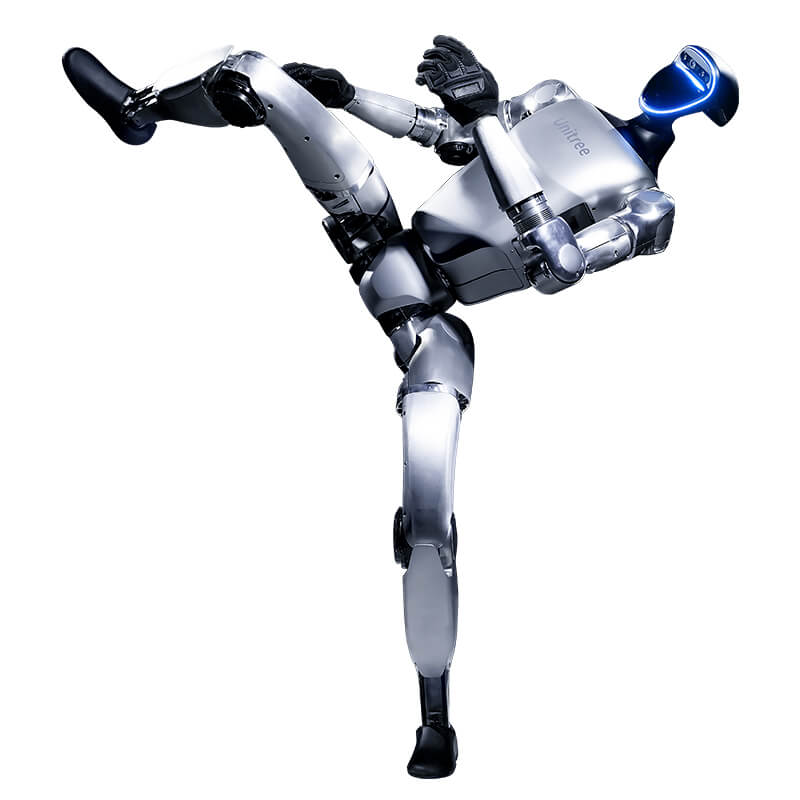
\includegraphics[width=0.25\linewidth]{immagini/Unitree_G1.jpg}
    \caption{Unitree G1. Fonte: \cite{unitreeManual2025}}
    \label{fig:G1}
\end{figure}

Scendendo nel dettaglio della sensoristica esterocettiva, la camera RGB-D montata è un'Intel RealSense D435i che integra un'unità di misura inerziale (IMU) a sei gradi di libertà\footnote{accelerometro a 3 assi e giroscopio a 3 assi}. La profondità non viene direttamente misurata da un sensore specifico ma calcolata utilizzando la visione stereoscopica. A partire dalle immagini di due camere parallele distanti $T$ (\textit{baseline}), si calcola la profondità grazie al teorema dei triangoli simili. Data la lunghezza focale $f$ e le coordinate dell'oggetto nelle immagini delle due camere ($x_r$ e $x_l$) si ricava la distanza $Z$ dell'oggetto dal \textit{piano della baseline} come segue:
\begin{equation}
    Z=f\frac{T}{x_l-x_r}
\end{equation}
Per utilizzare questa relazione è necessario individuare la corrispondenza tra i pixel delle due immagini che rappresentano lo stesso oggetto della scena. Questa procedura deve avvenire in maniera densa, ossia per ogni pixel. 

Questo permette una migliore comprensione del movimento e della posizione nello spazio. Il campo visivo secondo la scheda tecnica \cite{unitreeManual2025} ha una profondità di 87° in orizzontale e 58° in verticale. Il LiDAR, invece, è un LIVOX-MID360, compatto e ad alte prestazioni, progettato per applicazioni in robotica mobile, veicoli autonomi, droni e sistemi di mappatura. Sfrutta una tecnologia ibrida a stato solido con specchio rotante e offre una copertura a 360° in orizzontale e 59° in verticale. Il principio che regola il funzionamento del LiDAR è la misurazione del tempo di volo, ossia il calcolo della distanza $d$ di un oggetto nella scena a partire dal tempo $t$ impiegato dal fascio luminoso emesso dal sensore per colpirlo e tornare indietro. In particolare, la formula caratteristica, data la velocità della luce $c$, è la seguente:
\begin{equation}
    d = \frac{c\cdot t}{2}
\end{equation}
Lo stesso principio regola la misurazione laser semplice di cui il laser rappresenta un'evoluzione nella direzione di esaminare ambienti complessi attraverso più raggi luminosi o un unico raggio in movimento. La combinazione di LiDAR e camera RGB-D permette al robot di esaminare in maniera rapida e precisa l'ambiente circostante.

\begin{figure}[h]
    \centering
    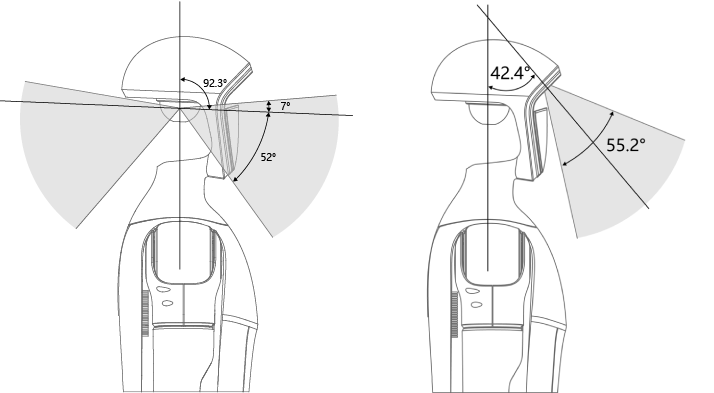
\includegraphics[width=0.5\linewidth]{immagini/sensori_g1.png}
    \caption{Angoli di visione del LiDAR (a sinistra) e della camera (a destra). Fonte: \cite{unitreeManual2025}}
    \label{fig:sensori_g1}
\end{figure}

% locomozione
Secondo il manuale di Unitree \cite{unitreeManual2025} l'umanoide ha a disposizione 12 gradi di libertà per la locomozione, entrambe le gambe sono provviste dei seguenti giunti rotanti e relativi limiti di movimento:

\begin{itemize}
    \item Roll per l'anca (-0,5236 $\sim$ 2,9671 rad)
    \item Pitch per l'anca (-2,5307 $\sim$ 2,8798 rad)
    \item Yaw per l'anca (-2,7576 $\sim$ 2,7576 rad)
    \item Ginocchio (-0,087267 $\sim$ 2,8798 rad)
    \item Pitch per la caviglia (-0,87267 $\sim$ 0,5236 rad)
    \item Roll per la caviglia (-0,2618 $\sim$ 0,2618 rad)
\end{itemize}

Le articolazioni del G1 utilizzano un motore sincrono a magneti permanenti sviluppato internamente da Unitree che eroga una coppia massima di 120 Nm\footnote{valore massimo tra tutti i motori presenti sul robot, corrispondente all'articolazione del ginocchio nella versione EDU} e presenta un design ad asse cavo che conferisce leggerezza e compattezza alla struttura. I giunti sono provvisti di encoder doppio che fornisce un feedback accurato di posizione e velocità, essenziale per il controllo di alta precisione. Tenuto conto delle limitazioni imposte per ragioni di sicurezza, il G1 raggiunge una velocità di 7 km/h, alla stregua della camminata umana.
